\documentclass[a4paper]{article}

\usepackage{fullpage} % Package to use full page
\usepackage{parskip} % Package to tweak paragraph skipping
\usepackage{tikz} % Package for drawing
\usepackage{amsmath}
\usepackage{hyperref}
\usepackage{enumitem}
\usepackage{mathtools}
\usepackage{subcaption}

\title{Scalable Machine Learning - Project Proposal}
\author{TheBrightSideOfLife: Giorgio Ruffa - Erik Wouters}
\date{17/01/2019}

\begin{document}

\maketitle

\section{Problem Description}
We aim to tackle a sound classification problem. 
More precisely, we want to distinguish if a determined sound sample belongs to a bee, a cricket or to ambient noise.
The problem is a classic fully supervised machine learning problem, where each instance of the data is already associated to a "ground truth" label.

\section{Tools}
We will use a Deep Learning approach, hence the following tools will be used: Tensorflow, Keras, Google CoLab or Hops Sites.

\section{Data}

The data is divided into two data sets: BUZZ1 and BUZZ2. The first one consists of $10260$ labeled audio samples taken in the same apiary roughly at the same time (2018). The second data set consists of $12914$ labeled audio samples. This data set is divided in a train and a validation set, where the validation set has data from a different apairy, different time (2017 vs. 2018) and a different bee race. Each of the audio samples is two seconds long. The data sets were downloaded from \url{https://usu.app.box.com/v/BeePiAudioData} \cite{BeePi} and a mirror can be found here: \url{https://erikwouters.stackstorage.com/s/rXj8xPLK8OwKIHE}.

\begin{figure}[ht]
  \centering
  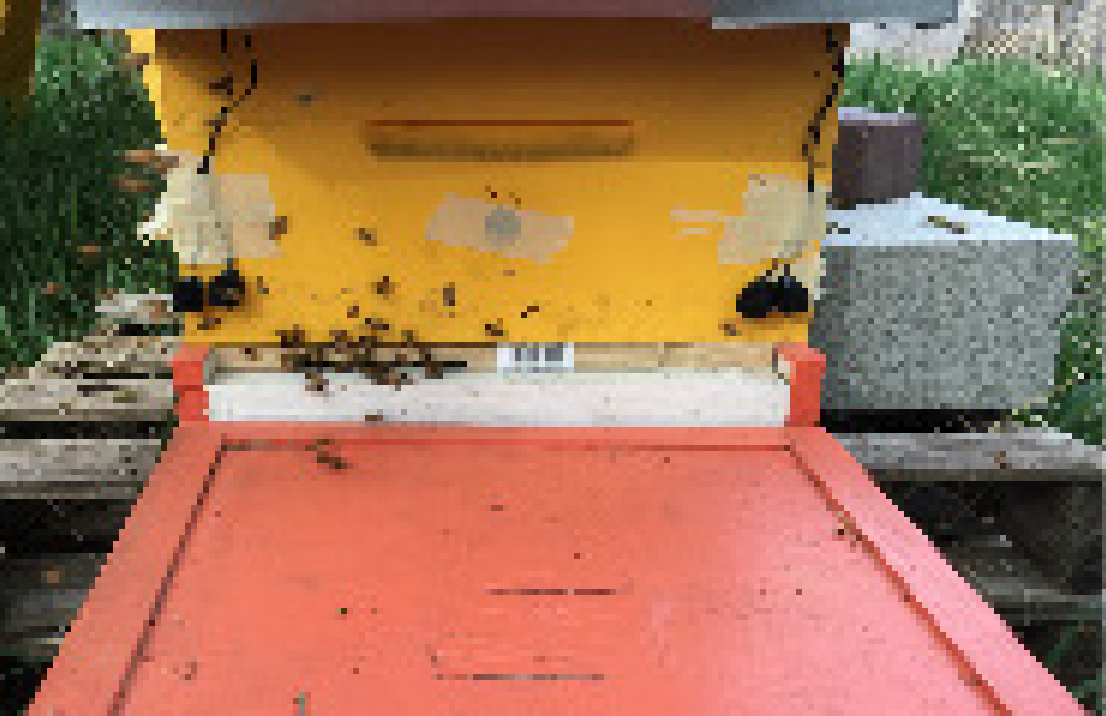
\includegraphics[scale=0.2]{Images/beepi_setup.png}
  \caption{Audio capture setup}
  \label{fig:beepi_setup}
\end{figure}

Each of the samples is labeled as either "bee", "cricket" or "noise".

\begin{figure}[!ht]
  \centering
  \begin{subfigure}[b]{0.32\textwidth}
    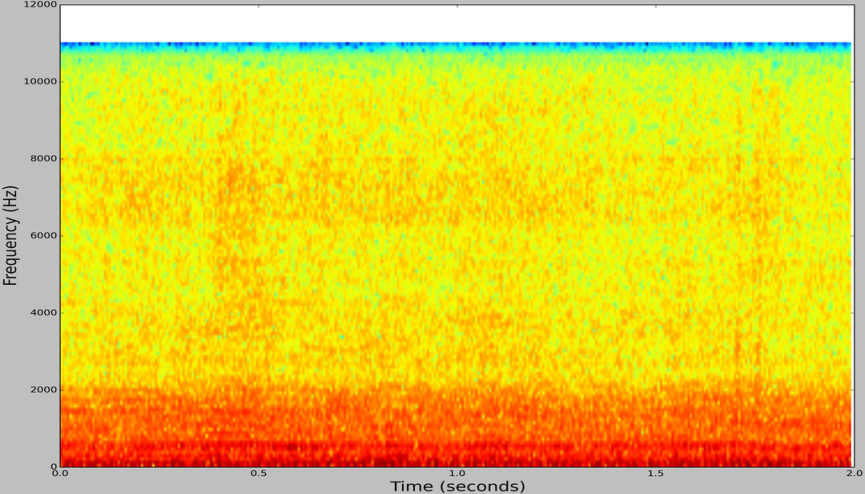
\includegraphics[width=\textwidth]{Images/spect_bee.png}
    \caption{Bee}
  \end{subfigure}
  \begin{subfigure}[b]{0.32\textwidth}
    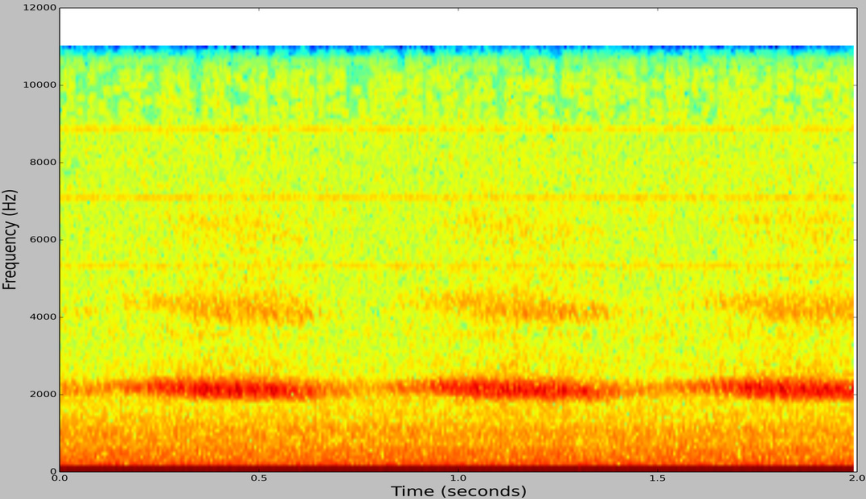
\includegraphics[width=\textwidth]{Images/spect_cricket.png}
    \caption{Cricket}
  \end{subfigure}
  \begin{subfigure}[b]{0.32\textwidth}
    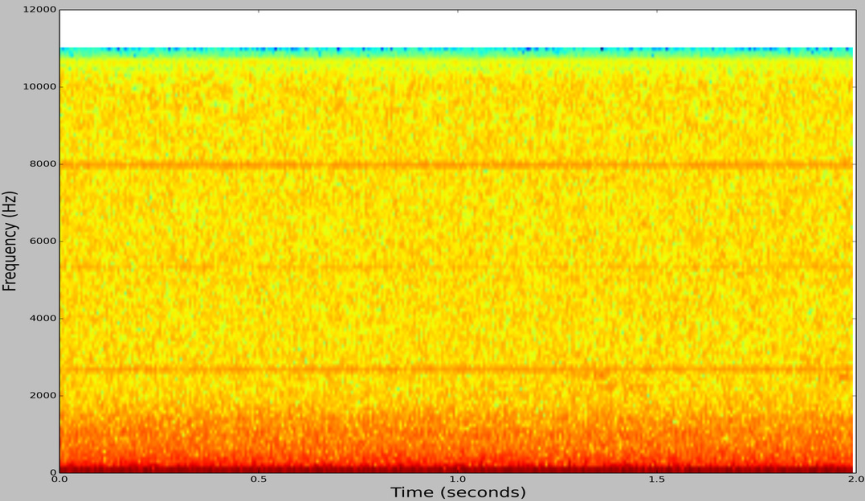
\includegraphics[width=\textwidth]{Images/spect_noise.png}
    \caption{Ambient noise}
  \end{subfigure}
  \caption{Spectrogram image of a sample from the three different classes \cite{Kulyukin}}
  \label{fig:spect}
\end{figure}


\section{Methodology}
The main idea is to represent each sample in form of a spectrogram. The spectrogram has on the x axis the time (usually milliseconds), while the y axis correspond to a frequency and the intensity of the frequency is encoded using a colormap (i.e. a scalar value). Thus spectrograms can be treated exactly as a grey-scale image.

Then the natural approach is to train a CNN model in a fully supervised way, using softmax cross-entropy as a loss function.

Metrics that can be used to evaluate the model are:
\begin{itemize}
    \item overall Accuracy
    \item class-wise precision and recall
    \item class-wise area under ROC curve
\end{itemize}


\bibliography{bibliography}{}
\bibliographystyle{plain}

\end{document}